\fxnote{Add interactive somewhere in the research question}
\fxnote{Who is the target audience?}
\chapter{Components of an interactive maps}
When creating an interactive map one must consider which features to add to enhance the user experience. To give an overview of some of the basic features used for navigating and get information from a map an example of an interactive map has been used. www.openstreetmap.org has been used as an example of an interactive map. \citep{OpenStreetMap} A picture of this map can be seen in figure \ref{InteractiveMap}. Its User Interface (UI) have been numbered with boxes, which have been colored green if the feature would make sense for exploring and comparing large population dataset. The reasoning behind the coloring is explained in section \ref{SortingFunctions}


\begin{figure} [H]
	\centering
	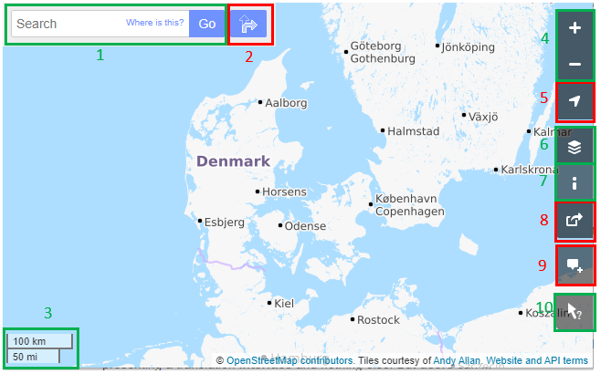
\includegraphics[width=.8\textwidth]{Pictures/InteractiveMap}
	\caption{An example of an interactive map}
	\label{InteractiveMap}
\end{figure}

\begin{table}[htbp]
	\centering
	\begin{tabular}{l}
		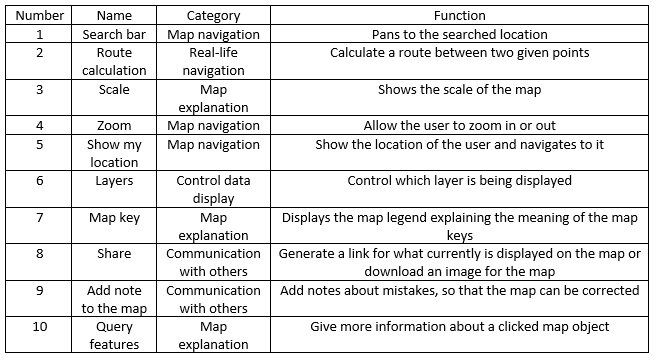
\includegraphics[width=0.8\textwidth]{Pictures/tabOSMFunctions}
	\end{tabular}
	\caption{Overview of the UI elements highlighted in figure \ref{InteractiveMap}}
	\label{tabOSMFunctions}
\end{table}

What the different parts of the UI does can be seen in table \ref{tabOSMFunctions}. The functions of the UI can be classified in five different categories. Using the map navigation UI the user can control which part of the map is being displayed.
The real-life navigation tool is used for navigating in the real world. 
The map explanation category gives the user information about the map. This can be general information about the scale or symbols on the map or specific information about a clicked point. 
The tool for controlling the displayed data is used for controlling what is being visualized on the map.
The last category, communication with others, is for sharing information with other users of the map. 
\fxnote{Write that my own search bar can be improved} 
\fxnote{Did I write about toogling dual legends?} 

\section{Relevant functionalities}\label{SortingFunctions}

Not all of these categories are relevant for this tool and this target audience. Most of the tools in the Map navigation category are relevant. Having a search bar allow the user to quickly pan to an area of interest and the zoom function allows the user to control the extent. The "Show my location" function is less relevant for this target audience. It would be relevant if the target audience was citizens, who just wanted to explore a population projection out of curiosity. These would potentially be interested in knowing what the expected population would be in their neighbourhood. If the researcher are working with the same area, where they happen to live they can pan to this area using the search bar. 

The Real-life navigation tool is only useful for route planning, which is not the purpose of this map. The map explanation tools are all useful for the application. 

%Having the scale gives the user a sense of scale, which is important especially in case the tool is being used in a part of the world which is unfamiliar to the user. 

While a scale can give the user a sense of scale, this is only useful if the scale is presented with a unit, which the user easily can comprehend. As mentioned in section x the unit of the projection is in degrees, which would result in the scale also being in degrees. It was therefore decided not to include a scale.
%While a scale can give the user a sense of scale, this is only useful if the scale is presented with a unit, which the user easily can comprehend. The scalebar in the figure is showing the distance in meters. This would not be the case, when visualising the population projections, since it is using degree as unit. Since this is not a commen scale measurement, the scale has been excluded. 
\fxnote{write about scale - update figure to exclude scale}

Having a legend is also central to explain the user which values the colors of the raster would correspond to. Getting more information about a clicked point could also be relevant for the tool. This information could be the exact value in the clicked point. The layer control is important, since this would allow the map to be able to display multiple different population projection.

The last category, Communication with others, is outside of the scope of this project, since these rely on multiple users. %Some of the functionalities of the share function could be useful for a single user. It could be relevant for the user to be able save different extents,


\fxnote{Update the figure to have the share box being relevant}

\fxnote{Write here if you come up with more relevant information, which you could throw in here}

\section{Comparing layers}

The functions presented so far does not enable an easy visual comparison of raster data. It is possible currently by changing back and forth between different layers with different population projections. This however is a bit inconvenient. 
An alternative way would be to use comparison layers in a similar fashion to how it currently is being done with the makeCityWebsite tool mentioned in section x. This would require the creation of comparison layers for each combination of SSPs and years, which should be compared.   
A third option would be to display multiple maps at the same time as illustrated in figure x. These two maps are linked together by a shared view. The means the panning or zooming in one map would do the same operation on the other map.

\begin{figure} [H]
	\centering
	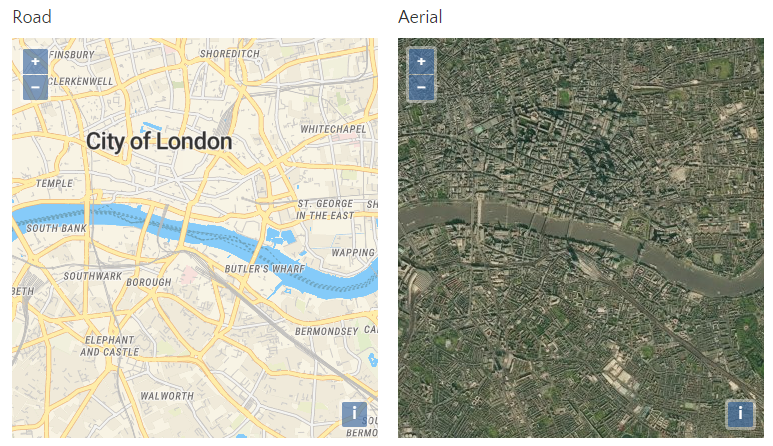
\includegraphics[width=.8\textwidth]{Pictures/DualMapExample}
	\caption{An example of two maps sharing the same view}
	\label{DualMapExample}
\end{figure}
https://openlayers.org/en/latest/examples/side-by-side.html

This third option was chosen.
 
\fxnote{Make frontpage}